% Commented out: 
% \addbibresource
% \includepdf

\documentclass[12pt,letterpaper,english,bibliography=totocnumbered, abstract=on]{scrartcl}

\usepackage{indentfirst}
\usepackage[titletoc]{appendix}
\usepackage{fullpage}
%\usepackage{subfiles}
\usepackage[T1]{fontenc}
\usepackage[latin9]{inputenc}
\usepackage{color}
\usepackage{babel}
\usepackage{verbatim}
\usepackage[unicode=true,pdfusetitle,
bookmarks=true,bookmarksnumbered=false,bookmarksopen=false,
breaklinks=true,pdfborder={0 0 0},pdfborderstyle={},backref=false,colorlinks=true]
{hyperref}
\hypersetup{linkcolor=blue,citecolor=blue,urlcolor=blue}

\usepackage{booktabs}
\usepackage{multirow}
\usepackage{adjustbox}
\usepackage{threeparttable}
\usepackage[table]{xcolor}
\usepackage{csquotes}
\usepackage{soul} % for hiliting text: \hl

\usepackage[backend=biber, style=authoryear, maxbibnames=99, dashed=false]{biblatex}
\setlength\bibitemsep{2\itemsep}
%\addbibresource{mylibrary.bib}
%\addbibresource{CRB.bib}

\usepackage{pdfpages}
\usepackage{float} % Allows use of H to place floats

\usepackage{pgfgantt}

\usepackage{framed}

% Prevent page breaks within paragraphs
% https://tex.stackexchange.com/questions/21983/how-to-avoid-page-breaks-inside-paragraphs
\widowpenalties 1 10000

\usepackage{subfig}

\begin{document}

\titlehead{DRAFT TECHNICAL REPORT}

\title{Automated Coconut Rhinoceros Beetle Roadside Damage Survey on Majuro, October 2023}

\author{Aubrey Moore PhD}

\date{December 1, 2023\\Revised December 12, 2023}

\maketitle

\footnote{\url{https://aubreymoore.github.io/Majuro-tech-report-20231201/Majuro-tech-report.pdf}}

%\newpage
%\tableofcontents

\pagebreak

\section{Methods}

A few days after coconut rhinoceros beetle was detected on Majuro, Christian Cayanan from the University of Guam visited the island to perform an automated roadside survey of CRB damage using methods developed on Guam. The survey was performed from 11 am and 3 pm on October 7, 2023. A smart phone programmed to record a georeferenced HD images at a rate of once per second was attached to the outside of a vehicle. The vehicle which was driven the eastern tip of the island to the western tip, returning along the same route. 13,488 roadside images were recorded.

These images were examined by a pair of object detectors, one which detected coconut palms and one which detected v-shaped cuts to fronds which are distinctive symptoms of CRB adult feeding damage. Results were reported in the form of an \href{https://aubreymoore.github.io/Majuro-CRB-Damage-Map-2023-10/webmap/#12/7.1098/171.2099}{interactive web map}. 

The original webmap reported a much higher level of damage on Majuro than expected. Examination of images showed that the object detectors were generating many false-positive detections. The detection threshold was increased from 50\% to 70\% for the coconut palm detector and from 50\% to 99\% for the v-shaped cut detector. In addition all detected v-shaped cuts were examined visually.

\section{Results and Discussion}

A \href{https://aubreymoore.github.io/Majuro-CRB-damage-map-1/webmap/#12/7.1082/171.2072}{revised interactive web map} has been generated. This map shows only 3 v-shaped cuts Fig. (\ref{fig:125004}, \ref{fig:125007}, \ref{fig:143930}), tightly clustered at a location just east of the airport (Fig. \ref{fig:v-cuts-location}).

At this point, the object detectors are not very efficient and results require validation by human observers viewing images or making field observations. The coconut palm detector makes few mistakes. But the v-shaped cut detector generates many false-positives and false-negatives. Further training and tuning of both detectors is needed. However, even in the current state, the methodology is still quite useful. Data acquisition is not a problem: acquiring 13,488 images required only 4 hours and the computer workflow reduced the human labor dramatically. It was not necessary to view 13,488 images, but only to validate a few hundred images selected by the object detectors. 

% TODO: \usepackage{graphicx} required
\begin{figure}
	\centering
	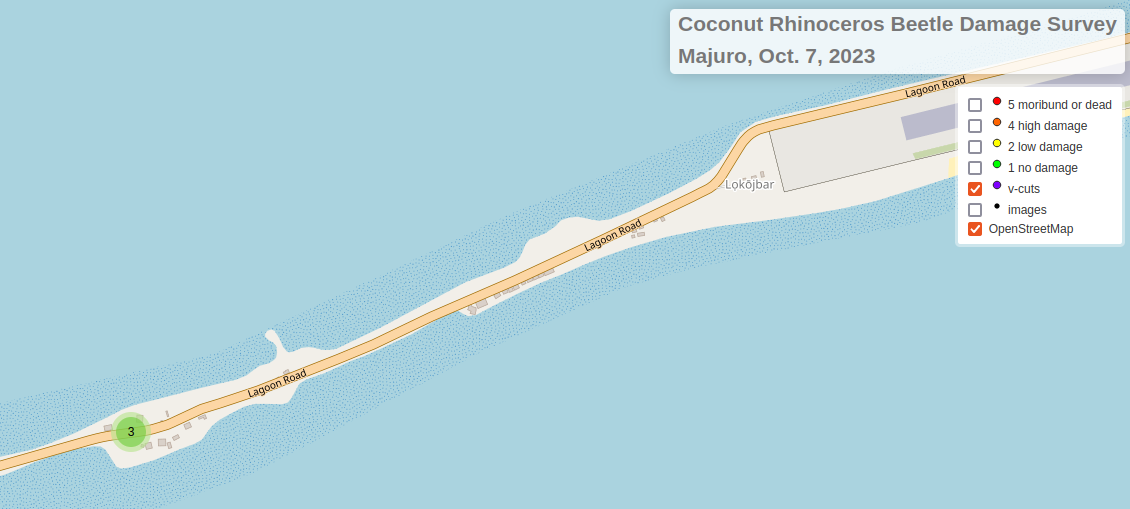
\includegraphics[width=\linewidth]{images/v-cuts-location}
	\caption{This screenshot of the web map shows the location of the cell phone  where 3 images containing v-cuts were detected.}
	\label{fig:v-cuts-location}
\end{figure}

% TODO: \usepackage{graphicx} required
\begin{figure}
	\centering
	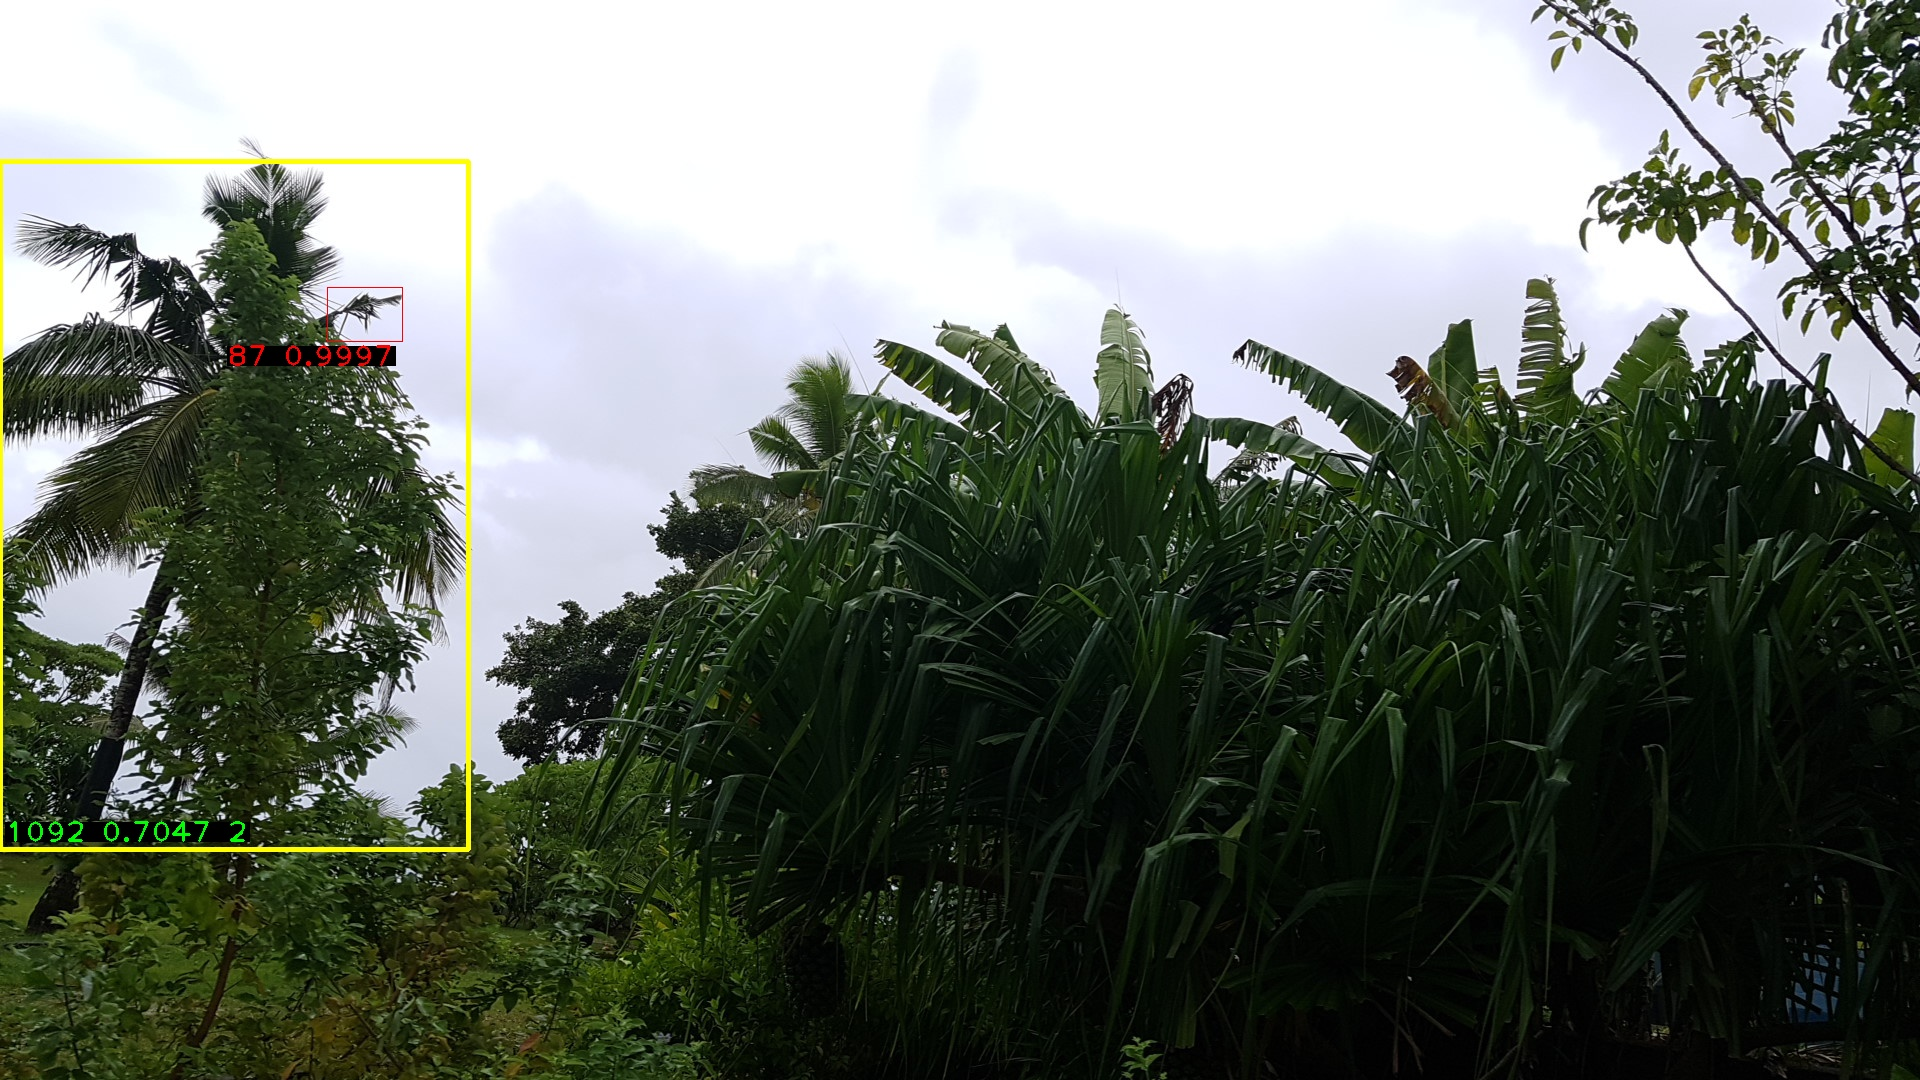
\includegraphics[width=\linewidth]{images/IMG_20231007_125004}
	\caption{Although only one v-shaped cut in the coconut on the left was detected, this tree has several other damage symptoms. Note that there is a second coconut palm to the right of this tree, almost occluded by banana and pandanus, which also has probable CRB damage.}
	\label{fig:125004}
\end{figure}

% TODO: \usepackage{graphicx} required
\begin{figure}
	\centering
	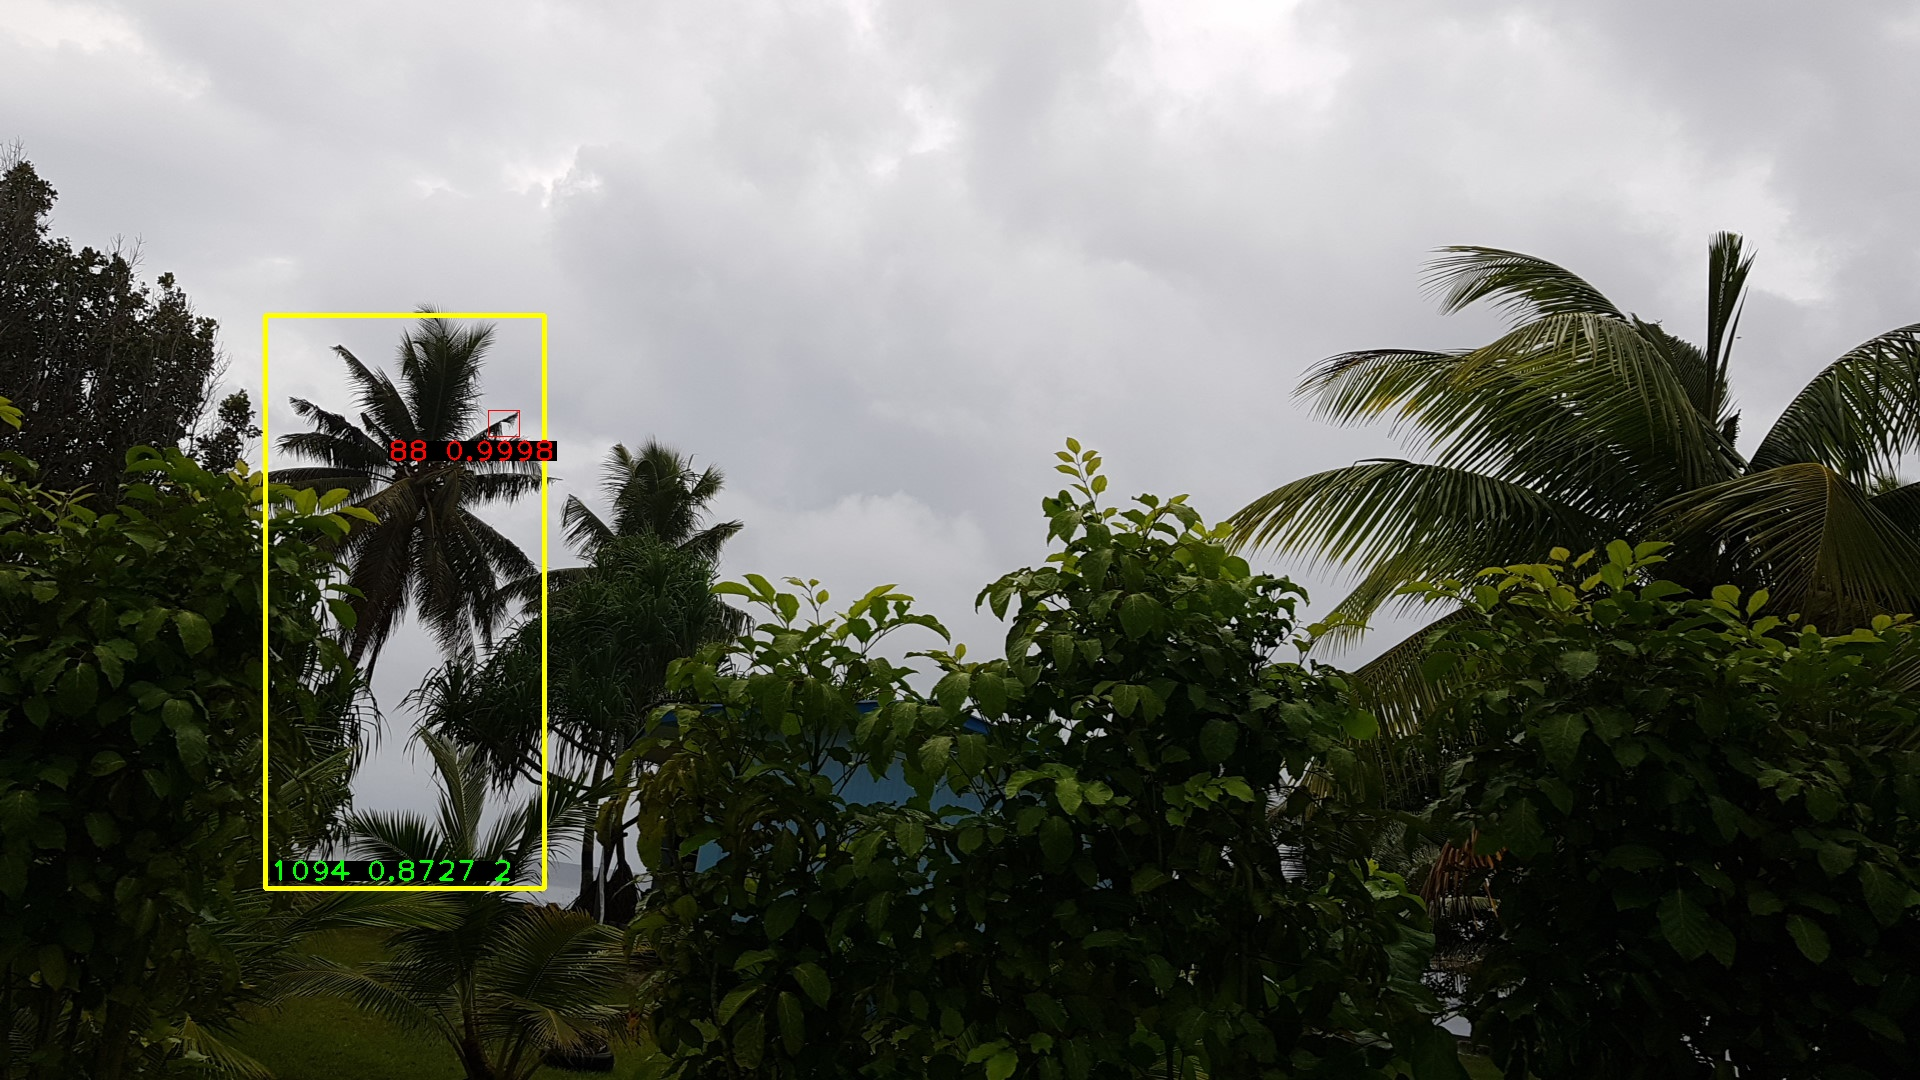
\includegraphics[width=\linewidth]{images/IMG_20231007_125007}
	\caption{This image was recorded just 3 seconds after the one shown in Fig. (\ref{fig:125007}). Note that the palm at the right of the image also shows CRB damage symptoms.}
	\label{fig:125007}
\end{figure}

% TODO: \usepackage{graphicx} required
\begin{figure}
	\centering
	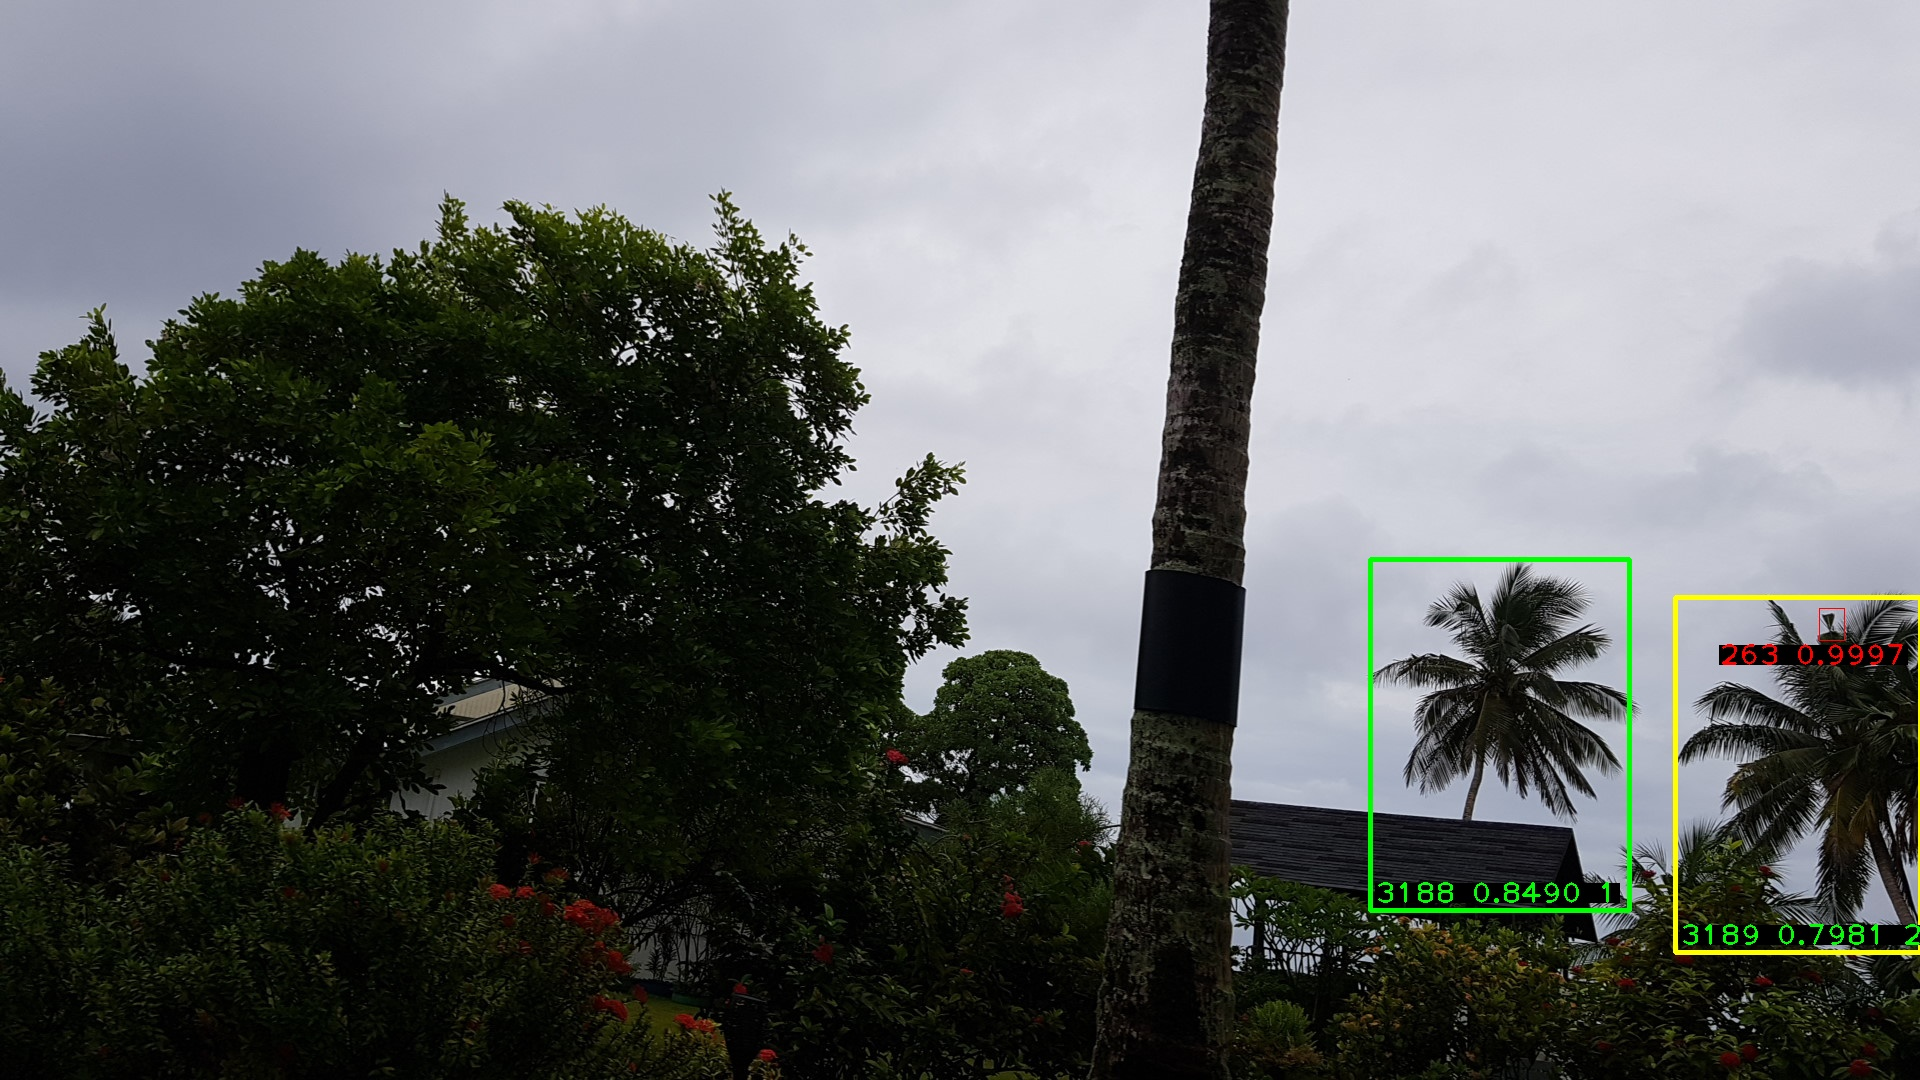
\includegraphics[width=\linewidth]{images/IMG_20231007_143930}
	\caption{This image, containing a v-shaped cut, was captured 1.5 h after the previous 2, on the return trip (from west to east). The damaged tree is on the south side of the road whereas the previous detections were on the north side of the road. }
	\label{fig:143930}
\end{figure}

\end{document}
